\section{Theorie}
\label{sec:Theorie}

Ein Lock-In Verstärker wird häufig verwendet, um verrauschte Signale zu messen,
indem eine zu messende Signalspannung mit einer Referenzspannung einer bestimmten
Frequenz $\omega_0$ moduliert wird.
Er besteht im Wesentlichen aus einem Bandpass, einem Phasenschieber, einem Mischer
und einem Tiefpassfilter. Der schematische Aufbau eines Lock-In Verstärkers ist
in \ref{fig:schema} zu sehen.

\begin{figure}
  \centering
  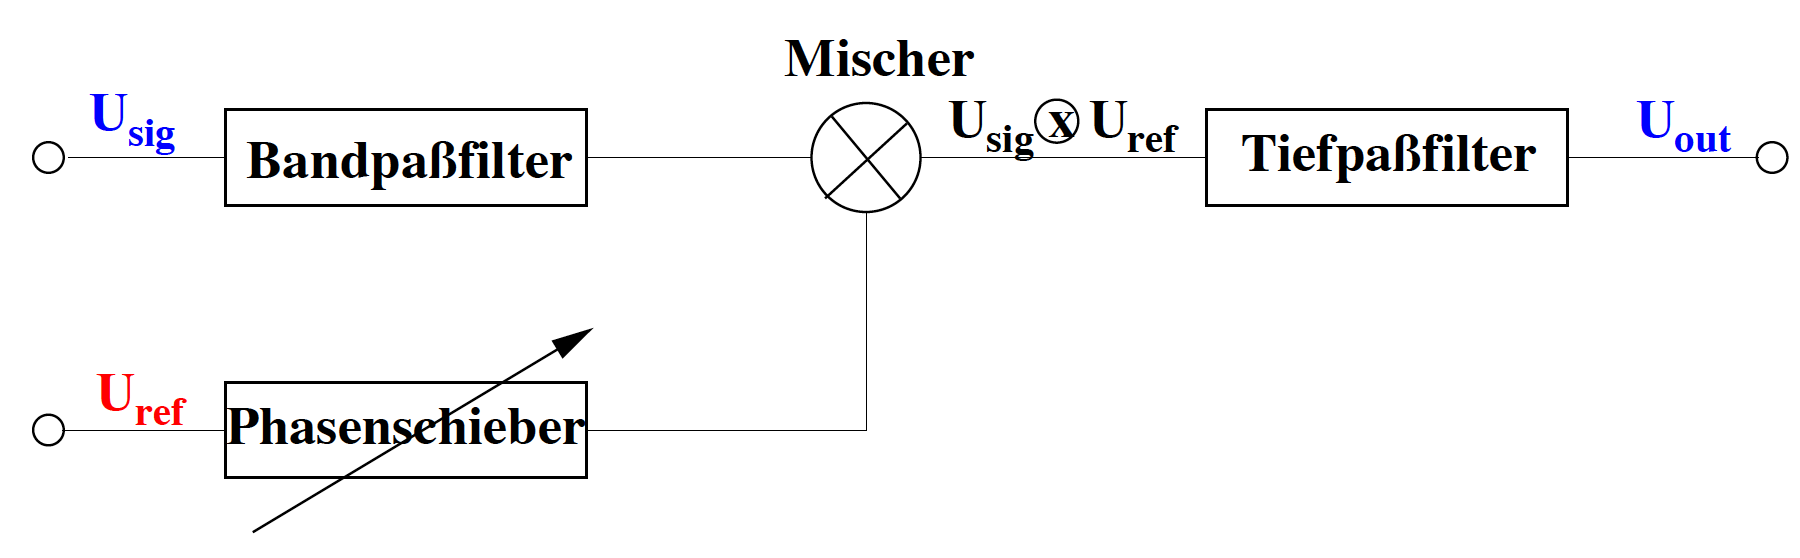
\includegraphics[width=\textwidth]{data/schema.png}
  \caption{Schematische Darstellung der Funktionsweise eines Lock-In Verstärkers
  \cite{Versuchsanleitung}}
  \label{fig:schema}
\end{figure}


Im Folgenden soll die Funktionsweise eines Lock-In Verstärkers kurz erläutert
werden. Im Bandpass werden zunächst sehr hohe und sehr tiefe Frequenzen der
Signalspannung $U_{\symup{sig}}$ herausfiltert. In einem Mischer wird die
Signalspannung $U_{\symup{sig}}$ mit einer Referenzspannung $U_{\symup{ref}}$
multipliziert. Dabei hat die Referenzspannung eine feste Kreisfrequenz
$\omega_0$ und eine durch einen Phasenschieber anpassbare Phase $\phi$. Die Phase
ist dabei so zu wählen, dass die Referenzspannung $U_{\symup{ref}}$ mit der
Signalspannung $U_{\symup{sig}}$ synchron verläuft. Das gemischte Signal wird
daraufhin in einem Tiefpass über mehrere Perioden integriert. Dabei muss darauf
geachtet werden, dass  die Zeitkonstante $\tau=RC$ des Tiefpasses viel kleiner
ist, als die Frequenz der Spannung. Dabei werden alle Frequenzen, die nicht
der synchronisierten Referenzfrequenz entsprechen, herausgefiltert und es entsteht
eine Ausgangsspannung $U_{\symup{out}}$, die Proportional zur Signalspannung
$U_{\symup{sig}}$ ist. Außerdem gilt für hinreichend große Integrationszeiten
der Zusammenhang
\begin{equation}
  U_{\symup{out}}\propto U_0 \cos(\phi) \,.
  \label{eqn:U_out_prop}
\end{equation}
An diesem Zusammenhang kann bereits erkannt werden, dass die Ausgangsspannung
$U_{\symup{out}}$ für eine Phase von $\phi=0$ maximal und für eine Phase von
$\phi=\frac{\pi}{2}$ null wird. 
Die Bandbreite $\Delta f$ des Restrauschens ist durch die Zeitkonstante $\tau$ des Tiefpasses
definiert. Sie folgt dem Zusammenhang
\begin{equation}
  \Delta f=\frac{1}{\pi R C} \,.
  \label{eqn:bandbreite}
\end{equation}
Wählt man die Zeitkonstante sehr groß, so können mit einem Lock-In Verstärker Güten
von bis zu $Q=100 \, 000$ erreicht werden.
Wird eine sinusförmige Signalspannung $U_{\symup{sig}}$ der Form
\begin{equation}
  U_{\symup{sig}}=U_{\symup{0}}\sin(\omega t)
\end{equation}
durch eine Referenzspannung $U_{\symup{ref}}$ derselben Frequenz moduliert, so
ergibt sich für die Ausgangsspannung nach der Integration durch den Tiefpass
der Zusammenhang
\begin{equation}
  U_{\symup{out}}=\frac{2}{\pi}U_{\symup{0}}\cos(\phi)\,.
\end{equation}
